% Options for packages loaded elsewhere
\PassOptionsToPackage{unicode}{hyperref}
\PassOptionsToPackage{hyphens}{url}
%
\documentclass[
]{article}
\usepackage{amsmath,amssymb}
\usepackage{iftex}
\ifPDFTeX
  \usepackage[T1]{fontenc}
  \usepackage[utf8]{inputenc}
  \usepackage{textcomp} % provide euro and other symbols
\else % if luatex or xetex
  \usepackage{unicode-math} % this also loads fontspec
  \defaultfontfeatures{Scale=MatchLowercase}
  \defaultfontfeatures[\rmfamily]{Ligatures=TeX,Scale=1}
\fi
\usepackage{lmodern}
\ifPDFTeX\else
  % xetex/luatex font selection
\fi
% Use upquote if available, for straight quotes in verbatim environments
\IfFileExists{upquote.sty}{\usepackage{upquote}}{}
\IfFileExists{microtype.sty}{% use microtype if available
  \usepackage[]{microtype}
  \UseMicrotypeSet[protrusion]{basicmath} % disable protrusion for tt fonts
}{}
\makeatletter
\@ifundefined{KOMAClassName}{% if non-KOMA class
  \IfFileExists{parskip.sty}{%
    \usepackage{parskip}
  }{% else
    \setlength{\parindent}{0pt}
    \setlength{\parskip}{6pt plus 2pt minus 1pt}}
}{% if KOMA class
  \KOMAoptions{parskip=half}}
\makeatother
\usepackage{xcolor}
\usepackage[margin=1in]{geometry}
\usepackage{color}
\usepackage{fancyvrb}
\newcommand{\VerbBar}{|}
\newcommand{\VERB}{\Verb[commandchars=\\\{\}]}
\DefineVerbatimEnvironment{Highlighting}{Verbatim}{commandchars=\\\{\}}
% Add ',fontsize=\small' for more characters per line
\usepackage{framed}
\definecolor{shadecolor}{RGB}{248,248,248}
\newenvironment{Shaded}{\begin{snugshade}}{\end{snugshade}}
\newcommand{\AlertTok}[1]{\textcolor[rgb]{0.94,0.16,0.16}{#1}}
\newcommand{\AnnotationTok}[1]{\textcolor[rgb]{0.56,0.35,0.01}{\textbf{\textit{#1}}}}
\newcommand{\AttributeTok}[1]{\textcolor[rgb]{0.13,0.29,0.53}{#1}}
\newcommand{\BaseNTok}[1]{\textcolor[rgb]{0.00,0.00,0.81}{#1}}
\newcommand{\BuiltInTok}[1]{#1}
\newcommand{\CharTok}[1]{\textcolor[rgb]{0.31,0.60,0.02}{#1}}
\newcommand{\CommentTok}[1]{\textcolor[rgb]{0.56,0.35,0.01}{\textit{#1}}}
\newcommand{\CommentVarTok}[1]{\textcolor[rgb]{0.56,0.35,0.01}{\textbf{\textit{#1}}}}
\newcommand{\ConstantTok}[1]{\textcolor[rgb]{0.56,0.35,0.01}{#1}}
\newcommand{\ControlFlowTok}[1]{\textcolor[rgb]{0.13,0.29,0.53}{\textbf{#1}}}
\newcommand{\DataTypeTok}[1]{\textcolor[rgb]{0.13,0.29,0.53}{#1}}
\newcommand{\DecValTok}[1]{\textcolor[rgb]{0.00,0.00,0.81}{#1}}
\newcommand{\DocumentationTok}[1]{\textcolor[rgb]{0.56,0.35,0.01}{\textbf{\textit{#1}}}}
\newcommand{\ErrorTok}[1]{\textcolor[rgb]{0.64,0.00,0.00}{\textbf{#1}}}
\newcommand{\ExtensionTok}[1]{#1}
\newcommand{\FloatTok}[1]{\textcolor[rgb]{0.00,0.00,0.81}{#1}}
\newcommand{\FunctionTok}[1]{\textcolor[rgb]{0.13,0.29,0.53}{\textbf{#1}}}
\newcommand{\ImportTok}[1]{#1}
\newcommand{\InformationTok}[1]{\textcolor[rgb]{0.56,0.35,0.01}{\textbf{\textit{#1}}}}
\newcommand{\KeywordTok}[1]{\textcolor[rgb]{0.13,0.29,0.53}{\textbf{#1}}}
\newcommand{\NormalTok}[1]{#1}
\newcommand{\OperatorTok}[1]{\textcolor[rgb]{0.81,0.36,0.00}{\textbf{#1}}}
\newcommand{\OtherTok}[1]{\textcolor[rgb]{0.56,0.35,0.01}{#1}}
\newcommand{\PreprocessorTok}[1]{\textcolor[rgb]{0.56,0.35,0.01}{\textit{#1}}}
\newcommand{\RegionMarkerTok}[1]{#1}
\newcommand{\SpecialCharTok}[1]{\textcolor[rgb]{0.81,0.36,0.00}{\textbf{#1}}}
\newcommand{\SpecialStringTok}[1]{\textcolor[rgb]{0.31,0.60,0.02}{#1}}
\newcommand{\StringTok}[1]{\textcolor[rgb]{0.31,0.60,0.02}{#1}}
\newcommand{\VariableTok}[1]{\textcolor[rgb]{0.00,0.00,0.00}{#1}}
\newcommand{\VerbatimStringTok}[1]{\textcolor[rgb]{0.31,0.60,0.02}{#1}}
\newcommand{\WarningTok}[1]{\textcolor[rgb]{0.56,0.35,0.01}{\textbf{\textit{#1}}}}
\usepackage{graphicx}
\makeatletter
\def\maxwidth{\ifdim\Gin@nat@width>\linewidth\linewidth\else\Gin@nat@width\fi}
\def\maxheight{\ifdim\Gin@nat@height>\textheight\textheight\else\Gin@nat@height\fi}
\makeatother
% Scale images if necessary, so that they will not overflow the page
% margins by default, and it is still possible to overwrite the defaults
% using explicit options in \includegraphics[width, height, ...]{}
\setkeys{Gin}{width=\maxwidth,height=\maxheight,keepaspectratio}
% Set default figure placement to htbp
\makeatletter
\def\fps@figure{htbp}
\makeatother
\setlength{\emergencystretch}{3em} % prevent overfull lines
\providecommand{\tightlist}{%
  \setlength{\itemsep}{0pt}\setlength{\parskip}{0pt}}
\setcounter{secnumdepth}{-\maxdimen} % remove section numbering
\ifLuaTeX
  \usepackage{selnolig}  % disable illegal ligatures
\fi
\IfFileExists{bookmark.sty}{\usepackage{bookmark}}{\usepackage{hyperref}}
\IfFileExists{xurl.sty}{\usepackage{xurl}}{} % add URL line breaks if available
\urlstyle{same}
\hypersetup{
  pdftitle={seesaw},
  hidelinks,
  pdfcreator={LaTeX via pandoc}}

\title{seesaw}
\author{}
\date{\vspace{-2.5em}}

\begin{document}
\maketitle

\begin{Shaded}
\begin{Highlighting}[]
\FunctionTok{library}\NormalTok{(seesaw)}
\FunctionTok{library}\NormalTok{(ggplot2)}
\FunctionTok{library}\NormalTok{(sf)}
\CommentTok{\#\textgreater{} Linking to GEOS 3.11.0, GDAL 3.5.3, PROJ 9.1.0; sf\_use\_s2() is TRUE}
\FunctionTok{library}\NormalTok{(GpGp)}
\end{Highlighting}
\end{Shaded}

\hypertarget{load-the-data}{%
\subsubsection{Load the Data}\label{load-the-data}}

\begin{Shaded}
\begin{Highlighting}[]

\FunctionTok{data}\NormalTok{(}\StringTok{"full\_table"}\NormalTok{, }\AttributeTok{package =} \StringTok{"seesaw"}\NormalTok{)}
\FunctionTok{data}\NormalTok{(}\StringTok{"station\_info"}\NormalTok{, }\AttributeTok{package =} \StringTok{"seesaw"}\NormalTok{)}
\FunctionTok{data}\NormalTok{(}\StringTok{"shp\_file"}\NormalTok{, }\AttributeTok{package =} \StringTok{"seesaw"}\NormalTok{)}
\FunctionTok{data}\NormalTok{(}\StringTok{"elevation\_grid"}\NormalTok{, }\AttributeTok{package =} \StringTok{"seesaw"}\NormalTok{)}
\FunctionTok{data}\NormalTok{(}\StringTok{"training\_X"}\NormalTok{, }\AttributeTok{package =} \StringTok{"seesaw"}\NormalTok{)}

\CommentTok{\# remove canadian NOAA stations}
\NormalTok{station\_info }\OtherTok{\textless{}{-}}\NormalTok{ station\_info[}\SpecialCharTok{!}\FunctionTok{is.na}\NormalTok{(station\_info}\SpecialCharTok{$}\NormalTok{state),]}
\end{Highlighting}
\end{Shaded}

\begin{enumerate}
\def\labelenumi{\arabic{enumi}.}
\tightlist
\item
  Make a map of the average temperature at each station for the month of
  March
\item
\end{enumerate}

\begin{Shaded}
\begin{Highlighting}[]
\CommentTok{\# Get list of station ids }
\NormalTok{station\_ids }\OtherTok{\textless{}{-}}\NormalTok{ station\_info}\SpecialCharTok{$}\NormalTok{station\_id}

\CommentTok{\# Filter data to include only March 2024, find average March 2024 }
\CommentTok{\# temperature for each station}
\NormalTok{march\_data }\OtherTok{\textless{}{-}}\NormalTok{ full\_table[full\_table}\SpecialCharTok{$}\NormalTok{LST\_DATE }\SpecialCharTok{\textgreater{}=} \StringTok{"2024{-}03{-}01"} 
                         \SpecialCharTok{\&}\NormalTok{ full\_table}\SpecialCharTok{$}\NormalTok{LST\_DATE }\SpecialCharTok{\textless{}=} \StringTok{"2024{-}03{-}31"}\NormalTok{, ]}

\CommentTok{\# Remove NAs}
\NormalTok{march\_data }\OtherTok{\textless{}{-}}\NormalTok{ march\_data[}\FunctionTok{complete.cases}\NormalTok{(march\_data), ]}

\NormalTok{average\_temps }\OtherTok{\textless{}{-}} \FunctionTok{aggregate}\NormalTok{(march\_data}\SpecialCharTok{$}\NormalTok{T\_DAILY\_AVG,}
                           \AttributeTok{by =} \FunctionTok{list}\NormalTok{( march\_data}\SpecialCharTok{$}\NormalTok{WBANNO ),}
                           \AttributeTok{FUN =}\NormalTok{ mean )}

\CommentTok{\# Create a new data frame with station ids, average temperatures,lat and lon}
\NormalTok{df }\OtherTok{\textless{}{-}} \FunctionTok{data.frame}\NormalTok{(}\AttributeTok{station\_id =} \FunctionTok{unique}\NormalTok{(march\_data}\SpecialCharTok{$}\NormalTok{WBANNO), }
                 \AttributeTok{average\_temp =}\NormalTok{ average\_temps}\SpecialCharTok{$}\NormalTok{x) }
\CommentTok{\# Merge df with station\_info to get lat and lon}
\NormalTok{df }\OtherTok{\textless{}{-}} \FunctionTok{merge}\NormalTok{(df, station\_info, }\AttributeTok{by.x =} \StringTok{"station\_id"}\NormalTok{, }\AttributeTok{by.y =} \StringTok{"station\_id"}\NormalTok{)}

\CommentTok{\# Drop NAs}
\NormalTok{df }\OtherTok{\textless{}{-}}\NormalTok{ df[}\FunctionTok{complete.cases}\NormalTok{(df), ]}

\CommentTok{\# Plot the USA shapefile and add the average temperature data as points}
\NormalTok{usa\_boundary }\OtherTok{\textless{}{-}} \FunctionTok{st\_crop}\NormalTok{(}\FunctionTok{st\_make\_valid}\NormalTok{(shp\_file), }\AttributeTok{xmin =} \SpecialCharTok{{-}}\DecValTok{125}\NormalTok{, }\AttributeTok{xmax =} \SpecialCharTok{{-}}\FloatTok{66.93457}\NormalTok{, }
                    \AttributeTok{ymin =} \FloatTok{22.396308}\NormalTok{, }\AttributeTok{ymax =} \FloatTok{49.384358}\NormalTok{)}
\CommentTok{\#\textgreater{} Warning: attribute variables are assumed to be spatially constant throughout}
\CommentTok{\#\textgreater{} all geometries}

\CommentTok{\# Convert the df to the right coordinate reference system}
\NormalTok{df\_sf }\OtherTok{\textless{}{-}} \FunctionTok{st\_as\_sf}\NormalTok{(df, }\AttributeTok{coords =} \FunctionTok{c}\NormalTok{(}\StringTok{"longitude"}\NormalTok{, }\StringTok{"latitude"}\NormalTok{), }\AttributeTok{crs =} 
                    \FunctionTok{st\_crs}\NormalTok{(usa\_boundary))}
\NormalTok{coordinates }\OtherTok{\textless{}{-}} \FunctionTok{st\_coordinates}\NormalTok{(df\_sf)}
\NormalTok{df\_sf}\SpecialCharTok{$}\NormalTok{x }\OtherTok{\textless{}{-}}\NormalTok{ coordinates[,}\DecValTok{1}\NormalTok{]}
\NormalTok{df\_sf}\SpecialCharTok{$}\NormalTok{y }\OtherTok{\textless{}{-}}\NormalTok{ coordinates[,}\DecValTok{2}\NormalTok{]}

\CommentTok{\# Use ggplot and sf to plot the map}
\FunctionTok{ggplot}\NormalTok{() }\SpecialCharTok{+}
  \FunctionTok{geom\_sf}\NormalTok{(}\AttributeTok{data =}\NormalTok{ usa\_boundary) }\SpecialCharTok{+}
  \FunctionTok{geom\_point}\NormalTok{(}\AttributeTok{data =}\NormalTok{ df\_sf, }\FunctionTok{aes}\NormalTok{(}\AttributeTok{color =}\NormalTok{ average\_temp, }\AttributeTok{x =}\NormalTok{ x, }\AttributeTok{y =}\NormalTok{ y), }\AttributeTok{size =} \DecValTok{1}\NormalTok{) }\SpecialCharTok{+}
  \FunctionTok{coord\_sf}\NormalTok{(}\AttributeTok{xlim =} \FunctionTok{c}\NormalTok{(}\SpecialCharTok{{-}}\DecValTok{125}\NormalTok{, }\SpecialCharTok{{-}}\FloatTok{66.93457}\NormalTok{), }\AttributeTok{ylim =} \FunctionTok{c}\NormalTok{(}\FloatTok{22.396308}\NormalTok{, }\FloatTok{49.384358}\NormalTok{)) }\SpecialCharTok{+}
  \FunctionTok{theme\_minimal}\NormalTok{() }\SpecialCharTok{+}
  \FunctionTok{labs}\NormalTok{(}\AttributeTok{title =} \StringTok{"Average Temperature for March 2024"}\NormalTok{, }
       \AttributeTok{x =} \StringTok{"Longitude"}\NormalTok{, }\AttributeTok{y =} \StringTok{"Latitude"}\NormalTok{) }\SpecialCharTok{+}
  \FunctionTok{scale\_color\_gradient}\NormalTok{(}\AttributeTok{name =} \StringTok{"Temperature (°C)"}\NormalTok{, }\AttributeTok{low =} \StringTok{"blue"}\NormalTok{, }\AttributeTok{high =} \StringTok{"red"}\NormalTok{) }\SpecialCharTok{+}
  \FunctionTok{theme}\NormalTok{(}\AttributeTok{plot.title =} \FunctionTok{element\_text}\NormalTok{(}\AttributeTok{hjust =} \FloatTok{0.5}\NormalTok{))}
\end{Highlighting}
\end{Shaded}

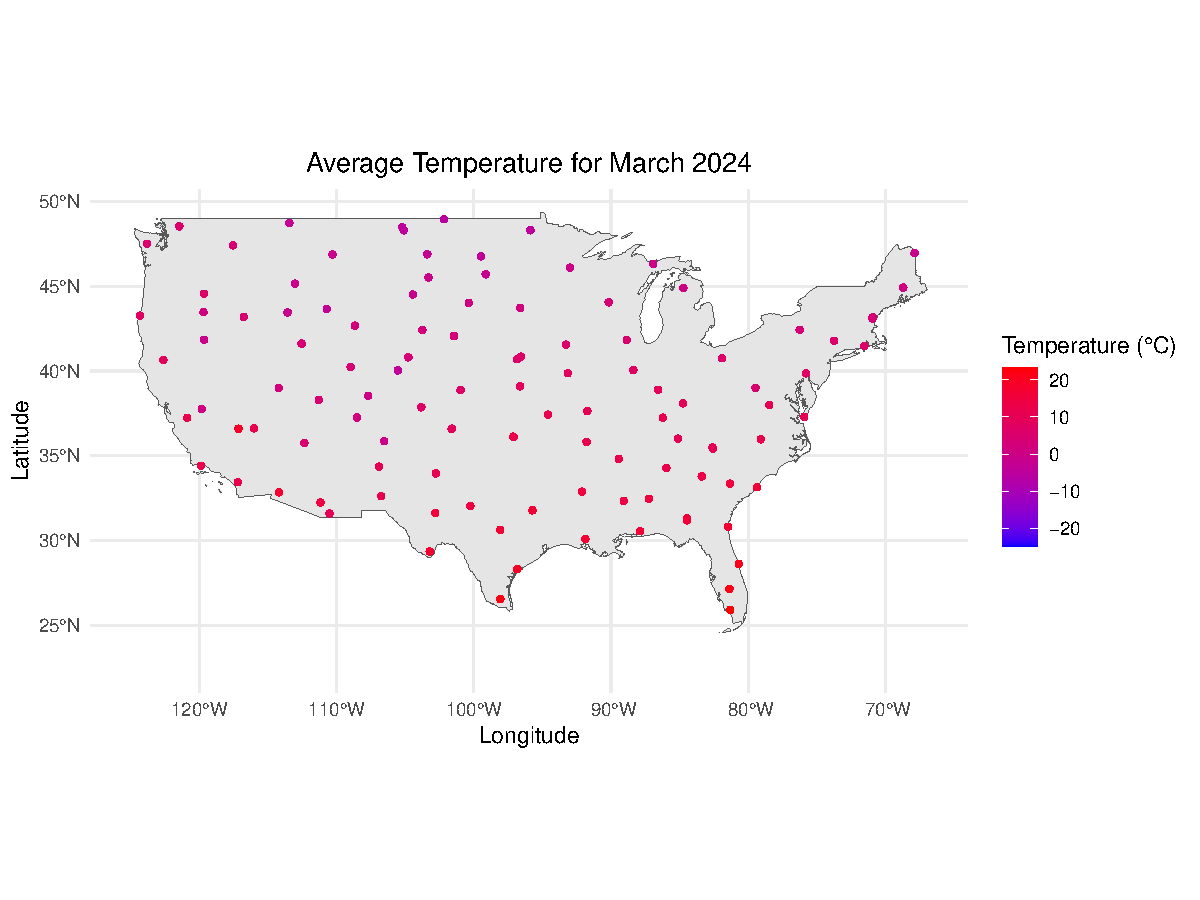
\includegraphics{seesaw_files/figure-latex/unnamed-chunk-3-1.pdf}

\begin{enumerate}
\def\labelenumi{\arabic{enumi}.}
\setcounter{enumi}{1}
\tightlist
\item
  Fit a spatial model and plot an interpolated map of average
  temperatures for March 2024. Consider including elevation in your
  model.
\end{enumerate}

A model without elevation:

\begin{Shaded}
\begin{Highlighting}[]
\CommentTok{\# Set up the grid for interpolation }
\NormalTok{res }\OtherTok{\textless{}{-}} \DecValTok{50}
\NormalTok{grid }\OtherTok{\textless{}{-}} \FunctionTok{usagrid}\NormalTok{(res)}

\CommentTok{\# Define the X and y to train the model }
\NormalTok{X }\OtherTok{\textless{}{-}} \FunctionTok{as.data.frame}\NormalTok{(}\FunctionTok{model.matrix}\NormalTok{(}\SpecialCharTok{\textasciitilde{}}\NormalTok{ x}\SpecialCharTok{+}\NormalTok{y , }\AttributeTok{data =}\NormalTok{ df\_sf))}
\NormalTok{y }\OtherTok{\textless{}{-}}\NormalTok{ df\_sf}\SpecialCharTok{$}\NormalTok{average\_temp}

\CommentTok{\# Use seesaw\textquotesingle{}s interpolate\_grid function to fit the spatial model}
\NormalTok{spatial\_model }\OtherTok{\textless{}{-}} \FunctionTok{interpolate\_grid}\NormalTok{(X,y,}\AttributeTok{resolution =}\NormalTok{ res)}
\CommentTok{\#\textgreater{} Assuming columns 1 and 2 of locs are (longitude,latidue) in degrees}

\FunctionTok{graph\_interp}\NormalTok{(spatial\_model, grid) }\SpecialCharTok{+} 
  \FunctionTok{labs}\NormalTok{( }\AttributeTok{title =} \StringTok{"Interpolated Average Temperatures for March 2024"}\NormalTok{,}
    \AttributeTok{x =} \StringTok{"Longitude"}\NormalTok{, }\AttributeTok{y =} \StringTok{"Latitude"}\NormalTok{, }
    \AttributeTok{fill =} \StringTok{"Temperature (°C)"}\NormalTok{)}
\end{Highlighting}
\end{Shaded}

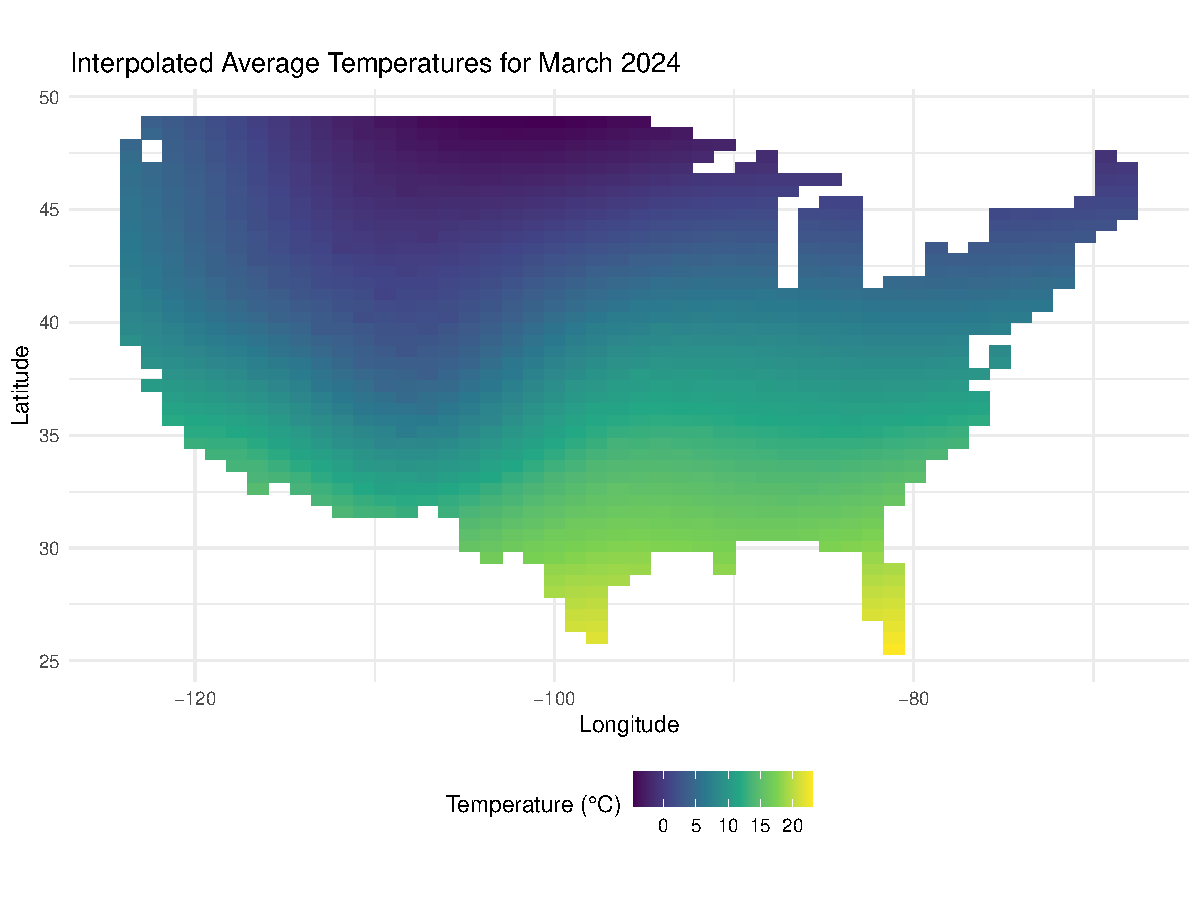
\includegraphics{seesaw_files/figure-latex/unnamed-chunk-4-1.pdf}

A model with elevation:

\begin{Shaded}
\begin{Highlighting}[]
\CommentTok{\# Fit a spatial model with elevation}
\NormalTok{locs }\OtherTok{\textless{}{-}}\NormalTok{ X[, }\FunctionTok{c}\NormalTok{(}\StringTok{"x"}\NormalTok{, }\StringTok{"y"}\NormalTok{)]}

\NormalTok{Xpred }\OtherTok{\textless{}{-}} \FunctionTok{as.data.frame}\NormalTok{(}\FunctionTok{model.matrix}\NormalTok{(}\SpecialCharTok{\textasciitilde{}}\NormalTok{ x}\SpecialCharTok{+}\NormalTok{y}\SpecialCharTok{+}\NormalTok{elevation, }\AttributeTok{data =}\NormalTok{ elevation\_grid))}
\CommentTok{\# Create model matrix}
\NormalTok{preds }\OtherTok{\textless{}{-}} \FunctionTok{interpolate\_grid}\NormalTok{(training\_X, y, }\AttributeTok{Xpred =}\NormalTok{ Xpred)}
\CommentTok{\#\textgreater{} Assuming columns 1 and 2 of locs are (longitude,latidue) in degrees}
\FunctionTok{graph\_interp}\NormalTok{(preds,grid) }\SpecialCharTok{+} 
  \FunctionTok{labs}\NormalTok{( }\AttributeTok{title =} \StringTok{"Interpolated Average Temperatures for March 2024 with Elevation"}\NormalTok{,}
    \AttributeTok{x =} \StringTok{"Longitude"}\NormalTok{, }\AttributeTok{y =} \StringTok{"Latitude"}\NormalTok{, }
    \AttributeTok{fill =} \StringTok{"Temperature (°C)"}\NormalTok{)}
\end{Highlighting}
\end{Shaded}

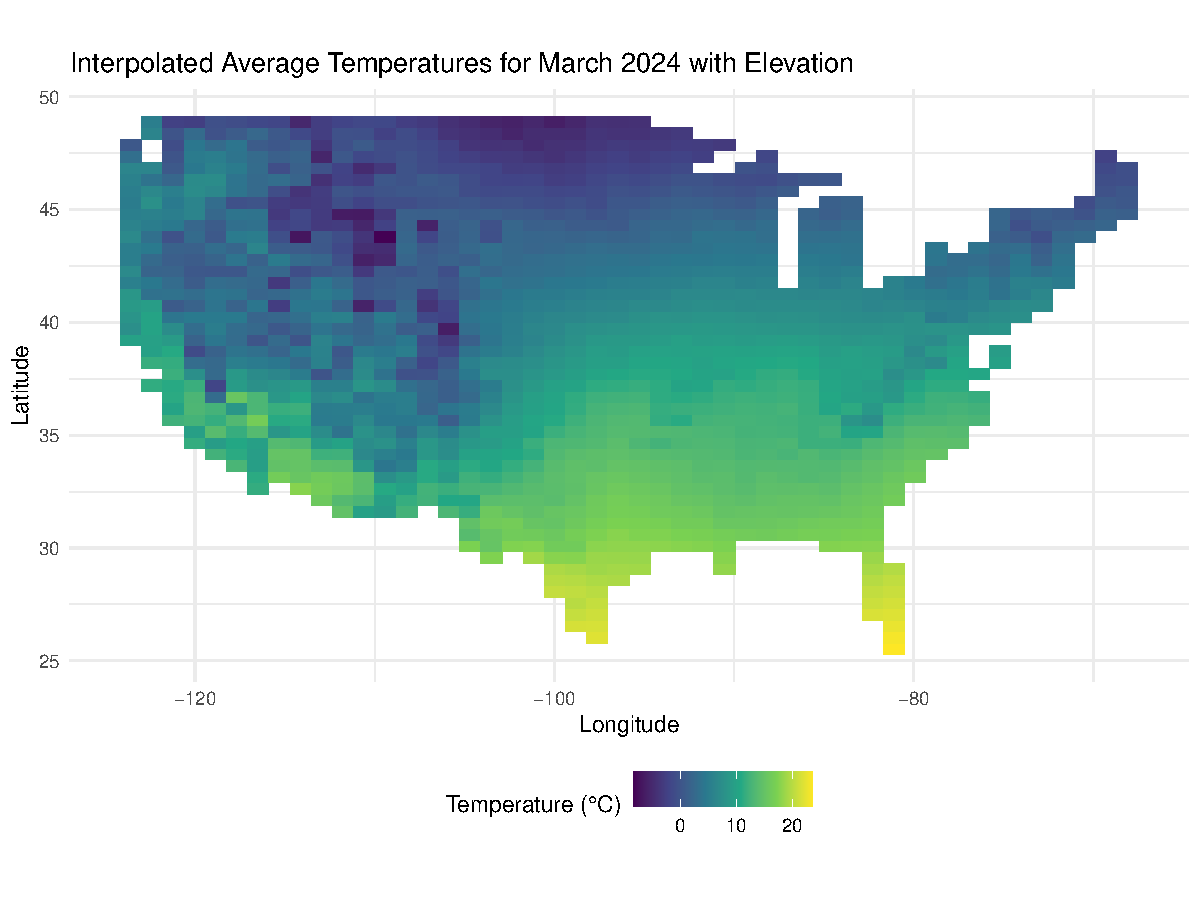
\includegraphics{seesaw_files/figure-latex/unnamed-chunk-5-1.pdf}

\begin{enumerate}
\def\labelenumi{\arabic{enumi}.}
\setcounter{enumi}{2}
\tightlist
\item
  Estimate the warmest and coldest day of the year for each station, and
  plot those days on two maps. Think carefully about how to represent
  the days numerically.
\end{enumerate}

In your report, describe the statistical analysis that you used for
estimating the warmest and coldest days at each station, including
writing down any statistical models in mathematical notation. Be sure to
define all your symbols and assumptions.

Interpolate maps of the warmest and coldest days, and plot the
interpolated maps of warmest and coldest days.

\begin{Shaded}
\begin{Highlighting}[]

\CommentTok{\# Create a function for finding the estimated warmest and coldest days of year}
\CommentTok{\# for a given station}
\NormalTok{warmest\_coldest }\OtherTok{\textless{}{-}} \ControlFlowTok{function}\NormalTok{(station\_id)\{}
\NormalTok{  cycle }\OtherTok{\textless{}{-}} \FunctionTok{yearly\_cycle\_station}\NormalTok{(station\_id, }\StringTok{"T\_DAILY\_AVG"}\NormalTok{)}
  \CommentTok{\#warmest\_day \textless{}{-} cycle$DOY[which.max(cycle$Expected\_T\_DAILY\_AVG)]}
\NormalTok{  warmest\_day }\OtherTok{\textless{}{-}} \FunctionTok{which.max}\NormalTok{(cycle}\SpecialCharTok{$}\NormalTok{Expected\_T\_DAILY\_AVG)}
  \CommentTok{\#coldest\_day \textless{}{-} cycle$DOY[which.min(cycle$Expected\_T\_DAILY\_AVG)]}
\NormalTok{  coldest\_day }\OtherTok{\textless{}{-}} \FunctionTok{which.min}\NormalTok{(cycle}\SpecialCharTok{$}\NormalTok{Expected\_T\_DAILY\_AVG)}
  \FunctionTok{return}\NormalTok{(}\FunctionTok{c}\NormalTok{(warmest\_day, coldest\_day))}
\NormalTok{\}}

\CommentTok{\# Preallocate the data frame}
\NormalTok{warmest\_coldest\_days }\OtherTok{\textless{}{-}} \FunctionTok{data.frame}\NormalTok{(}\AttributeTok{station\_id =}\NormalTok{ station\_ids, }
                                   \AttributeTok{warmest\_day =} \FunctionTok{integer}\NormalTok{(}\FunctionTok{length}\NormalTok{(station\_ids)), }
                                   \AttributeTok{coldest\_day =} \FunctionTok{integer}\NormalTok{(}\FunctionTok{length}\NormalTok{(station\_ids)))}

\CommentTok{\# Loop through each station}
\ControlFlowTok{for}\NormalTok{ (i }\ControlFlowTok{in} \DecValTok{1}\SpecialCharTok{:}\FunctionTok{length}\NormalTok{(station\_ids))\{}
  \CommentTok{\# Assign values directly without using c()}
\NormalTok{  warmest\_coldest\_days[i, }\FunctionTok{c}\NormalTok{(}\StringTok{"warmest\_day"}\NormalTok{, }\StringTok{"coldest\_day"}\NormalTok{)] }\OtherTok{\textless{}{-}} 
    \FunctionTok{warmest\_coldest}\NormalTok{(station\_ids[i])}
\NormalTok{\}}

\CommentTok{\# Use sf to get the correct coordinate reference system to plot }
\NormalTok{df\_warmest\_coldest }\OtherTok{\textless{}{-}} \FunctionTok{merge}\NormalTok{(warmest\_coldest\_days, station\_info, }
                    \AttributeTok{by.x =} \StringTok{"station\_id"}\NormalTok{, }\AttributeTok{by.y =} \StringTok{"station\_id"}\NormalTok{)}
\NormalTok{df\_warm\_cold\_sf }\OtherTok{\textless{}{-}} \FunctionTok{st\_as\_sf}\NormalTok{(df\_warmest\_coldest, }
                          \AttributeTok{coords =} \FunctionTok{c}\NormalTok{(}\StringTok{"longitude"}\NormalTok{, }\StringTok{"latitude"}\NormalTok{), }
                          \AttributeTok{crs =} \FunctionTok{st\_crs}\NormalTok{(usa\_boundary))}

\NormalTok{coordinates }\OtherTok{\textless{}{-}} \FunctionTok{st\_coordinates}\NormalTok{(df\_warm\_cold\_sf)}
\NormalTok{df\_warm\_cold\_sf}\SpecialCharTok{$}\NormalTok{x }\OtherTok{\textless{}{-}}\NormalTok{ coordinates[,}\DecValTok{1}\NormalTok{]}
\NormalTok{df\_warm\_cold\_sf}\SpecialCharTok{$}\NormalTok{y }\OtherTok{\textless{}{-}}\NormalTok{ coordinates[,}\DecValTok{2}\NormalTok{]}

\CommentTok{\# Plot the warmest day }
\FunctionTok{ggplot}\NormalTok{() }\SpecialCharTok{+}
  \FunctionTok{geom\_sf}\NormalTok{(}\AttributeTok{data =}\NormalTok{ usa\_boundary) }\SpecialCharTok{+}
  \FunctionTok{coord\_sf}\NormalTok{(}\AttributeTok{lims\_method =} \StringTok{"geometry\_bbox"}\NormalTok{) }\SpecialCharTok{+}
  \FunctionTok{geom\_point}\NormalTok{(}\AttributeTok{data =}\NormalTok{ df\_warm\_cold\_sf, }
             \FunctionTok{aes}\NormalTok{(}\AttributeTok{color =}\NormalTok{ warmest\_day, }\AttributeTok{x =}\NormalTok{ x, }\AttributeTok{y =}\NormalTok{ y), }\AttributeTok{size =} \DecValTok{1}\NormalTok{) }\SpecialCharTok{+}
  \FunctionTok{theme\_minimal}\NormalTok{() }\SpecialCharTok{+}
  \FunctionTok{labs}\NormalTok{(}\AttributeTok{title =} \StringTok{"Warmest Day of the Year for Each Station"}\NormalTok{, }
       \AttributeTok{x =} \StringTok{"Longitude"}\NormalTok{, }\AttributeTok{y =} \StringTok{"Latitude"}\NormalTok{) }\SpecialCharTok{+}
  \FunctionTok{scale\_color\_gradient}\NormalTok{(}\AttributeTok{name =} \StringTok{"Day of Year"}\NormalTok{, }
                       \AttributeTok{labels =} \FunctionTok{c}\NormalTok{(}\StringTok{"Jun 23"}\NormalTok{, }\StringTok{"Jul 1"}\NormalTok{, }\StringTok{"Jul 15"}\NormalTok{, }\StringTok{"Jul 31"}\NormalTok{, }
                                  \StringTok{"Aug 15"}\NormalTok{, }\StringTok{"Aug 30"}\NormalTok{), }
                       \AttributeTok{breaks =} \FunctionTok{c}\NormalTok{(}\DecValTok{174}\NormalTok{, }\DecValTok{184}\NormalTok{, }\DecValTok{196}\NormalTok{, }\DecValTok{212}\NormalTok{, }\DecValTok{227}\NormalTok{, }\DecValTok{242}\NormalTok{), }
                       \AttributeTok{trans =} \StringTok{"reverse"}\NormalTok{, }\AttributeTok{low =} \StringTok{"blue"}\NormalTok{, }\AttributeTok{high =} \StringTok{"red"}\NormalTok{) }\SpecialCharTok{+}
  \FunctionTok{guides}\NormalTok{(}\AttributeTok{colour =} \FunctionTok{guide\_colourbar}\NormalTok{(}\AttributeTok{title.vjust =} \FloatTok{1.5}\NormalTok{)) }\SpecialCharTok{+}
  \FunctionTok{theme}\NormalTok{(}\AttributeTok{plot.title =} \FunctionTok{element\_text}\NormalTok{(}\AttributeTok{hjust =} \FloatTok{0.5}\NormalTok{))}
\end{Highlighting}
\end{Shaded}

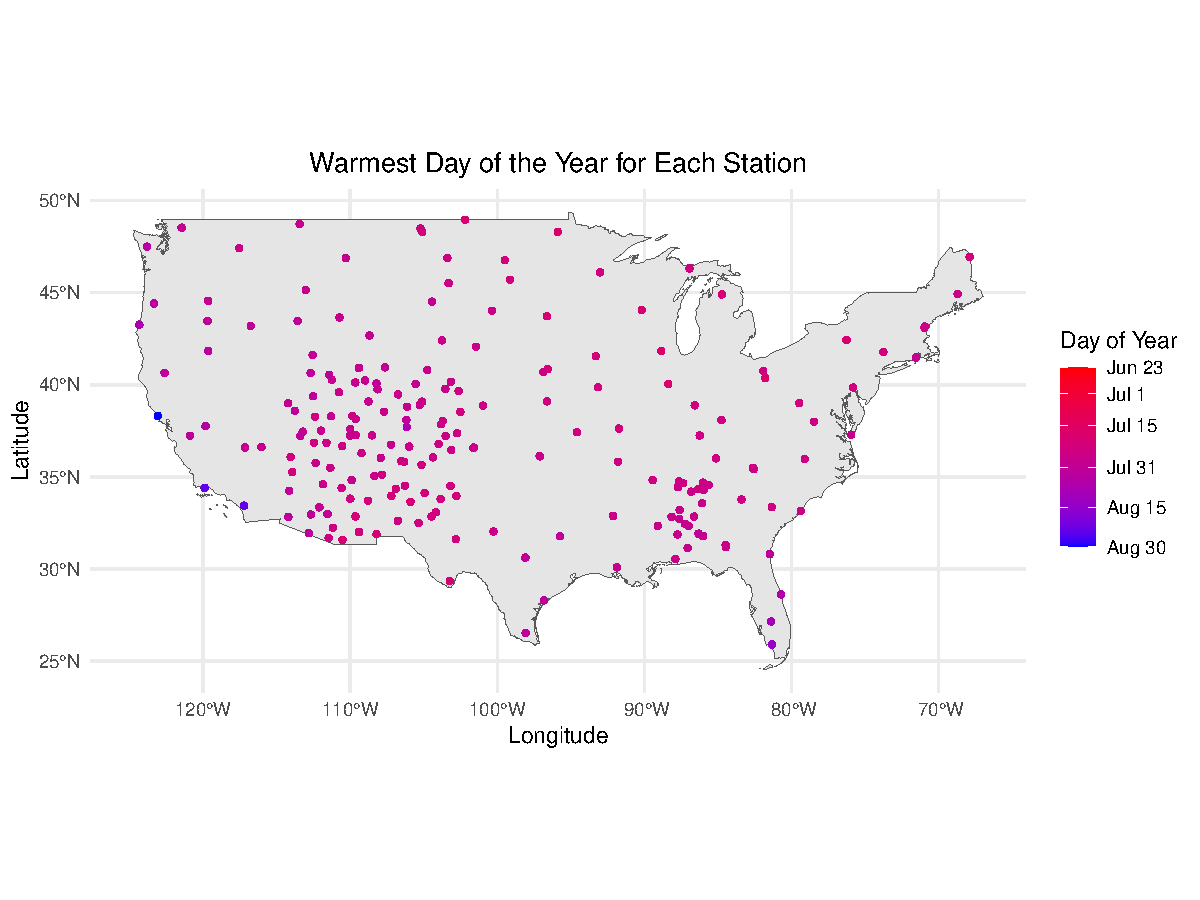
\includegraphics{seesaw_files/figure-latex/unnamed-chunk-6-1.pdf}

\begin{Shaded}
\begin{Highlighting}[]

\CommentTok{\# Function to map days from December 1st to January 31st to a continuous scale}
\NormalTok{day\_to\_continuous\_scale }\OtherTok{\textless{}{-}} \ControlFlowTok{function}\NormalTok{(day) \{}
  \ControlFlowTok{if}\NormalTok{ (day }\SpecialCharTok{\textless{}=} \DecValTok{31}\NormalTok{) \{}
    \FunctionTok{return}\NormalTok{(day }\SpecialCharTok{+} \DecValTok{31}\NormalTok{)}
\NormalTok{  \} }\ControlFlowTok{else}\NormalTok{ \{}
    \FunctionTok{return}\NormalTok{(}\DecValTok{31} \SpecialCharTok{{-}}\NormalTok{ (}\DecValTok{365}\SpecialCharTok{{-}}\NormalTok{day)}\SpecialCharTok{/}\DecValTok{31}\NormalTok{)}
\NormalTok{  \}}
\NormalTok{\}}

\CommentTok{\# Apply the function to the coldest day data}
\NormalTok{df\_warm\_cold\_sf}\SpecialCharTok{$}\NormalTok{continuous\_day }\OtherTok{\textless{}{-}} \FunctionTok{sapply}\NormalTok{(df\_warm\_cold\_sf}\SpecialCharTok{$}\NormalTok{coldest\_day, }
\NormalTok{                                         day\_to\_continuous\_scale)}

\CommentTok{\# Plot the shapefile and add the coldest day data as points}
\FunctionTok{ggplot}\NormalTok{() }\SpecialCharTok{+}
  \FunctionTok{geom\_sf}\NormalTok{(}\AttributeTok{data =}\NormalTok{ usa\_boundary) }\SpecialCharTok{+}
  \FunctionTok{coord\_sf}\NormalTok{(}\AttributeTok{lims\_method =} \StringTok{"geometry\_bbox"}\NormalTok{) }\SpecialCharTok{+}
  \FunctionTok{geom\_point}\NormalTok{(}\AttributeTok{data =}\NormalTok{ df\_warm\_cold\_sf, }
             \FunctionTok{aes}\NormalTok{(}\AttributeTok{color =}\NormalTok{ continuous\_day, }\AttributeTok{x =}\NormalTok{ x, }\AttributeTok{y =}\NormalTok{ y), }\AttributeTok{size =} \DecValTok{1}\NormalTok{) }\SpecialCharTok{+}
  \FunctionTok{scale\_color\_gradient}\NormalTok{(}\AttributeTok{name =} \StringTok{"Day of Year"}\NormalTok{,}
                       \AttributeTok{labels =} \FunctionTok{c}\NormalTok{(}\StringTok{"Dec 21"}\NormalTok{, }\StringTok{"Jan 1"}\NormalTok{, }\StringTok{"Jan 15"}\NormalTok{, }\StringTok{"Jan 30"}\NormalTok{),}
                       \AttributeTok{breaks =} \FunctionTok{c}\NormalTok{(}\DecValTok{21}\NormalTok{, }\DecValTok{32}\NormalTok{, }\DecValTok{46}\NormalTok{, }\DecValTok{62}\NormalTok{),}
                       \AttributeTok{trans =} \StringTok{"reverse"}\NormalTok{, }\AttributeTok{low =} \StringTok{"blue"}\NormalTok{, }\AttributeTok{high =} \StringTok{"red"}\NormalTok{) }\SpecialCharTok{+}
  \FunctionTok{theme\_minimal}\NormalTok{() }\SpecialCharTok{+}
  \FunctionTok{labs}\NormalTok{(}\AttributeTok{title =} \StringTok{"Coldest Day of the Year for Each Station"}\NormalTok{, }
       \AttributeTok{x =} \StringTok{"Longitude"}\NormalTok{, }\AttributeTok{y =} \StringTok{"Latitude"}\NormalTok{) }\SpecialCharTok{+} 
  \FunctionTok{guides}\NormalTok{(}\AttributeTok{colour =} \FunctionTok{guide\_colourbar}\NormalTok{(}\AttributeTok{title.vjust =} \FloatTok{1.5}\NormalTok{)) }\SpecialCharTok{+}
  \FunctionTok{theme}\NormalTok{(}\AttributeTok{plot.title =} \FunctionTok{element\_text}\NormalTok{(}\AttributeTok{hjust =} \FloatTok{0.5}\NormalTok{))}
\end{Highlighting}
\end{Shaded}

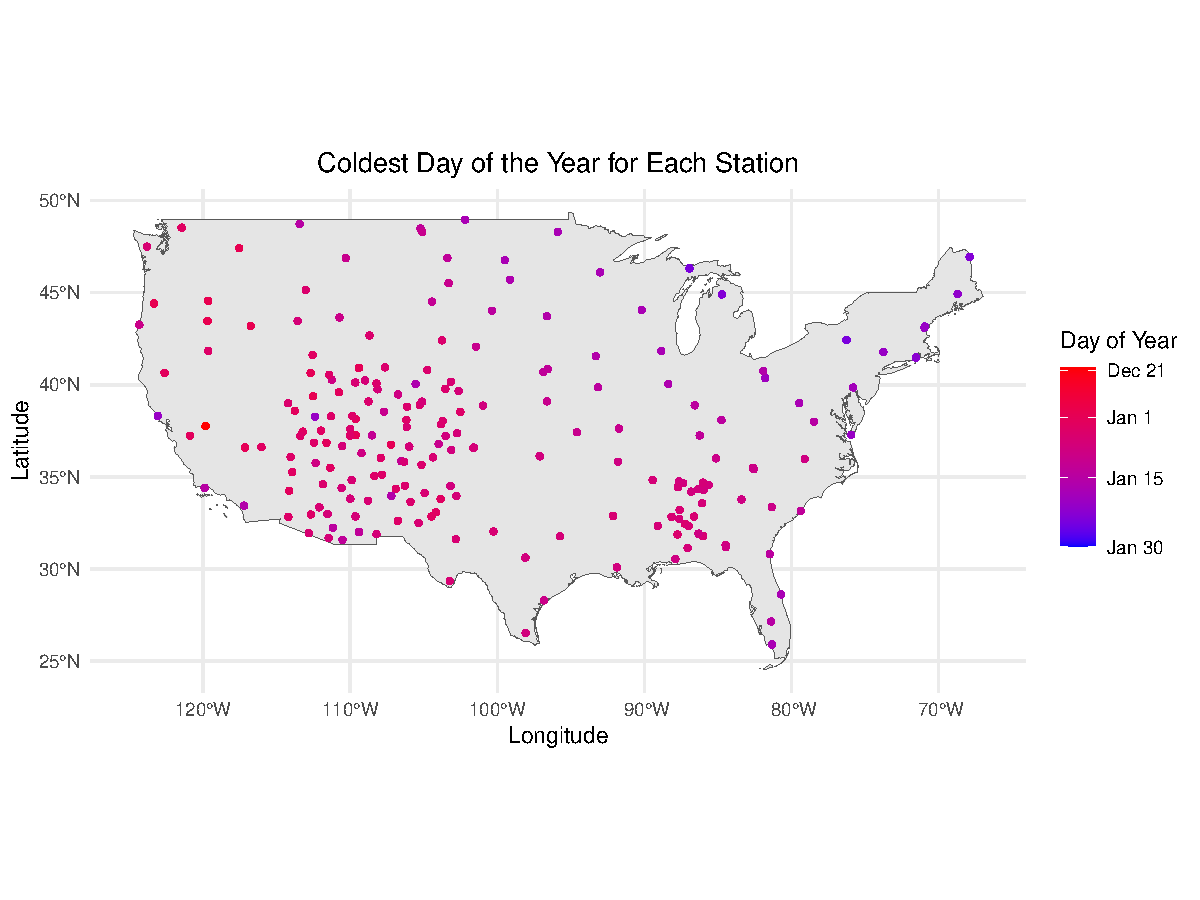
\includegraphics{seesaw_files/figure-latex/unnamed-chunk-7-1.pdf}

Statistical Model:

The estimated average warmest and coldest day of the year was calculated
by fitting a sinusoidal model to the daily average temperature data for
each station. The model is given by:

\(Y_i = \beta_0 + \beta_1 * \sin(2\pi d/365) + \beta_2*\cos(2\pi d/365) + \epsilon_i\)

where \(Y_i\) is the daily average temperature, \(d\) is the day of the
year, and \(\epsilon_i\) is the error term. The estimated warmest day of
the year is the day with the highest expected temperature, and the
estimated coldest day of the year is the day with the lowest expected
temperature.

Assumptions: 1. The daily average temperature data is sinusoidal with a
period of 365 days. 2. The daily average temperature data is stationary
over time. 3. The error term is normally distributed with mean 0 and
constant variance.

\begin{Shaded}
\begin{Highlighting}[]
\CommentTok{\# Create higher resolution grid }
\NormalTok{res }\OtherTok{\textless{}{-}} \DecValTok{200}
\NormalTok{grid }\OtherTok{\textless{}{-}} \FunctionTok{usagrid}\NormalTok{(res)}

\CommentTok{\# Ensure correct types}
\NormalTok{df\_warmest\_coldest}\SpecialCharTok{$}\NormalTok{rescaled\_coldest }\OtherTok{\textless{}{-}} 
  \FunctionTok{as.numeric}\NormalTok{(df\_warm\_cold\_sf}\SpecialCharTok{$}\NormalTok{continuous\_day)}
\NormalTok{df\_warmest\_coldest}\SpecialCharTok{$}\NormalTok{longitude }\OtherTok{\textless{}{-}} \FunctionTok{as.numeric}\NormalTok{(df\_warmest\_coldest}\SpecialCharTok{$}\NormalTok{longitude)}
\NormalTok{df\_warmest\_coldest}\SpecialCharTok{$}\NormalTok{latitude }\OtherTok{\textless{}{-}} \FunctionTok{as.numeric}\NormalTok{(df\_warmest\_coldest}\SpecialCharTok{$}\NormalTok{latitude)}
\NormalTok{locs }\OtherTok{\textless{}{-}}\NormalTok{ df\_warmest\_coldest[, }\FunctionTok{c}\NormalTok{(}\StringTok{"longitude"}\NormalTok{, }\StringTok{"latitude"}\NormalTok{)]}

\CommentTok{\# Make a dataframes of locations and y\_cold/y\_warm}
\NormalTok{cold\_dataset }\OtherTok{\textless{}{-}}\NormalTok{ df\_warmest\_coldest[,}\FunctionTok{c}\NormalTok{(}\StringTok{"longitude"}\NormalTok{, }\StringTok{"latitude"}\NormalTok{, }
                                      \StringTok{"rescaled\_coldest"}\NormalTok{)]}
\NormalTok{warm\_dataset }\OtherTok{\textless{}{-}}\NormalTok{ df\_warmest\_coldest[,}\FunctionTok{c}\NormalTok{(}\StringTok{"longitude"}\NormalTok{, }\StringTok{"latitude"}\NormalTok{, }\StringTok{"warmest\_day"}\NormalTok{)]}

\CommentTok{\# Drop repeated rows}
\NormalTok{cold\_dataset }\OtherTok{\textless{}{-}}\NormalTok{ cold\_dataset[}\SpecialCharTok{!}\FunctionTok{duplicated}\NormalTok{(cold\_dataset),]}
\NormalTok{warm\_dataset }\OtherTok{\textless{}{-}}\NormalTok{ warm\_dataset[}\SpecialCharTok{!}\FunctionTok{duplicated}\NormalTok{(warm\_dataset),]}

\CommentTok{\# Set up X and y for the interpolation }
\NormalTok{X\_cold }\OtherTok{\textless{}{-}} \FunctionTok{as.data.frame}\NormalTok{(}\FunctionTok{cbind}\NormalTok{(}\DecValTok{1}\NormalTok{, cold\_dataset[, }\FunctionTok{c}\NormalTok{(}\StringTok{"longitude"}\NormalTok{, }\StringTok{"latitude"}\NormalTok{)]))}
\FunctionTok{names}\NormalTok{(X\_cold) }\OtherTok{\textless{}{-}} \FunctionTok{c}\NormalTok{(}\StringTok{"intercept"}\NormalTok{, }\StringTok{"x"}\NormalTok{, }\StringTok{"y"}\NormalTok{)}
\NormalTok{X\_warm }\OtherTok{\textless{}{-}} \FunctionTok{as.data.frame}\NormalTok{(}\FunctionTok{cbind}\NormalTok{(}\DecValTok{1}\NormalTok{, warm\_dataset[, }\FunctionTok{c}\NormalTok{(}\StringTok{"longitude"}\NormalTok{, }\StringTok{"latitude"}\NormalTok{)]))}
\FunctionTok{names}\NormalTok{(X\_warm) }\OtherTok{\textless{}{-}} \FunctionTok{c}\NormalTok{(}\StringTok{"intercept"}\NormalTok{, }\StringTok{"x"}\NormalTok{, }\StringTok{"y"}\NormalTok{)}
\NormalTok{y\_cold }\OtherTok{\textless{}{-}}\NormalTok{ cold\_dataset}\SpecialCharTok{$}\NormalTok{rescaled\_coldest}
\NormalTok{y\_warm }\OtherTok{\textless{}{-}}\NormalTok{ warm\_dataset}\SpecialCharTok{$}\NormalTok{warmest\_day}

\CommentTok{\# Run the interpolations }
\NormalTok{warm\_pred }\OtherTok{\textless{}{-}} \FunctionTok{interpolate\_grid}\NormalTok{(X\_warm, y\_warm, }\AttributeTok{resolution =}\NormalTok{ res)}
\CommentTok{\#\textgreater{} Assuming columns 1 and 2 of locs are (longitude,latidue) in degrees}
\NormalTok{cold\_pred }\OtherTok{\textless{}{-}} \FunctionTok{interpolate\_grid}\NormalTok{(X\_cold,y\_cold, }\AttributeTok{resolution =}\NormalTok{ res)}
\CommentTok{\#\textgreater{} Assuming columns 1 and 2 of locs are (longitude,latidue) in degrees}

\CommentTok{\# Plot interpolations}
\FunctionTok{graph\_interp}\NormalTok{(warm\_pred, grid) }\SpecialCharTok{+} 
  \FunctionTok{labs}\NormalTok{( }\AttributeTok{title =} \StringTok{"Interpolated Warmest Day of the Year"}\NormalTok{,}
    \AttributeTok{x =} \StringTok{"Longitude"}\NormalTok{, }\AttributeTok{y =} \StringTok{"Latitude"}\NormalTok{, }
    \AttributeTok{fill =} \StringTok{"Day of Year"}\NormalTok{) }\SpecialCharTok{+}
\FunctionTok{scale\_fill\_gradient}\NormalTok{(}\AttributeTok{name =} \StringTok{"Day of Year"}\NormalTok{, }
                    \AttributeTok{labels =} \FunctionTok{c}\NormalTok{(}\StringTok{"Jul 21"}\NormalTok{, }\StringTok{"Jul 31"}\NormalTok{, }\StringTok{"Aug 10"}\NormalTok{, }\StringTok{"Aug 20"}\NormalTok{), }
                       \AttributeTok{breaks =} \FunctionTok{c}\NormalTok{(}\DecValTok{202}\NormalTok{, }\DecValTok{212}\NormalTok{, }\DecValTok{222}\NormalTok{, }\DecValTok{232}\NormalTok{), }
                    \AttributeTok{low =} \StringTok{"blue"}\NormalTok{, }\AttributeTok{high =} \StringTok{"red"}\NormalTok{, }
                    \AttributeTok{trans =} \StringTok{"reverse"}\NormalTok{) }\SpecialCharTok{+}
  \FunctionTok{guides}\NormalTok{(}\AttributeTok{colour =} \FunctionTok{guide\_colourbar}\NormalTok{(}\AttributeTok{title.vjust =} \FloatTok{1.5}\NormalTok{)) }\SpecialCharTok{+}
  \FunctionTok{theme}\NormalTok{(}\AttributeTok{legend.position =} \StringTok{"right"}\NormalTok{)}
\CommentTok{\#\textgreater{} Scale for fill is already present.}
\CommentTok{\#\textgreater{} Adding another scale for fill, which will replace the existing scale.}
\end{Highlighting}
\end{Shaded}

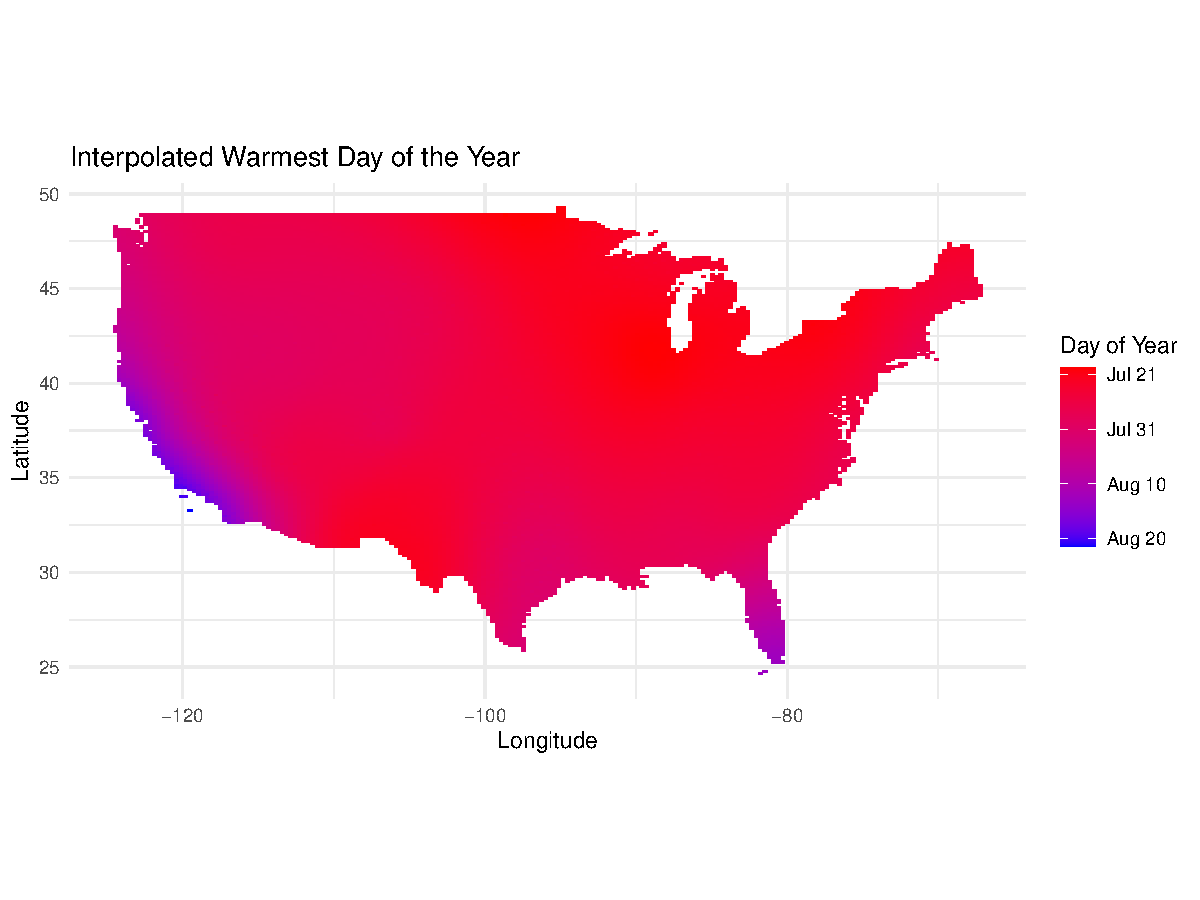
\includegraphics{seesaw_files/figure-latex/unnamed-chunk-8-1.pdf}

\begin{Shaded}
\begin{Highlighting}[]

\FunctionTok{graph\_interp}\NormalTok{(cold\_pred, grid) }\SpecialCharTok{+} 
  \FunctionTok{labs}\NormalTok{( }\AttributeTok{title =} \StringTok{"Interpolated Coldest Day of the Year"}\NormalTok{,}
    \AttributeTok{x =} \StringTok{"Longitude"}\NormalTok{, }\AttributeTok{y =} \StringTok{"Latitude"}\NormalTok{, }
    \AttributeTok{fill =} \StringTok{"Day of Year"}\NormalTok{) }\SpecialCharTok{+} 
  \FunctionTok{scale\_fill\_gradient}\NormalTok{(}\AttributeTok{name =} \StringTok{"Day of Year"}\NormalTok{, }
                      \AttributeTok{labels =} \FunctionTok{c}\NormalTok{(}\StringTok{"Dec 20"}\NormalTok{, }\StringTok{"Jan 1"}\NormalTok{, }\StringTok{"Jan 14"}\NormalTok{, }\StringTok{"Jan 25"}\NormalTok{),}
                       \AttributeTok{breaks =} \FunctionTok{c}\NormalTok{(}\DecValTok{21}\NormalTok{, }\DecValTok{32}\NormalTok{, }\DecValTok{45}\NormalTok{, }\FloatTok{55.8}\NormalTok{),}
                      \AttributeTok{low =} \StringTok{"blue"}\NormalTok{, }\AttributeTok{high =} \StringTok{"red"}\NormalTok{, }\AttributeTok{trans =} \StringTok{"reverse"}\NormalTok{)  }\SpecialCharTok{+}
  \FunctionTok{guides}\NormalTok{(}\AttributeTok{colour =} \FunctionTok{guide\_colourbar}\NormalTok{(}\AttributeTok{title.vjust =} \FloatTok{1.5}\NormalTok{)) }\SpecialCharTok{+}
  \FunctionTok{theme}\NormalTok{(}\AttributeTok{legend.position =} \StringTok{"right"}\NormalTok{)}
\CommentTok{\#\textgreater{} Scale for fill is already present.}
\CommentTok{\#\textgreater{} Adding another scale for fill, which will replace the existing scale.}
\end{Highlighting}
\end{Shaded}

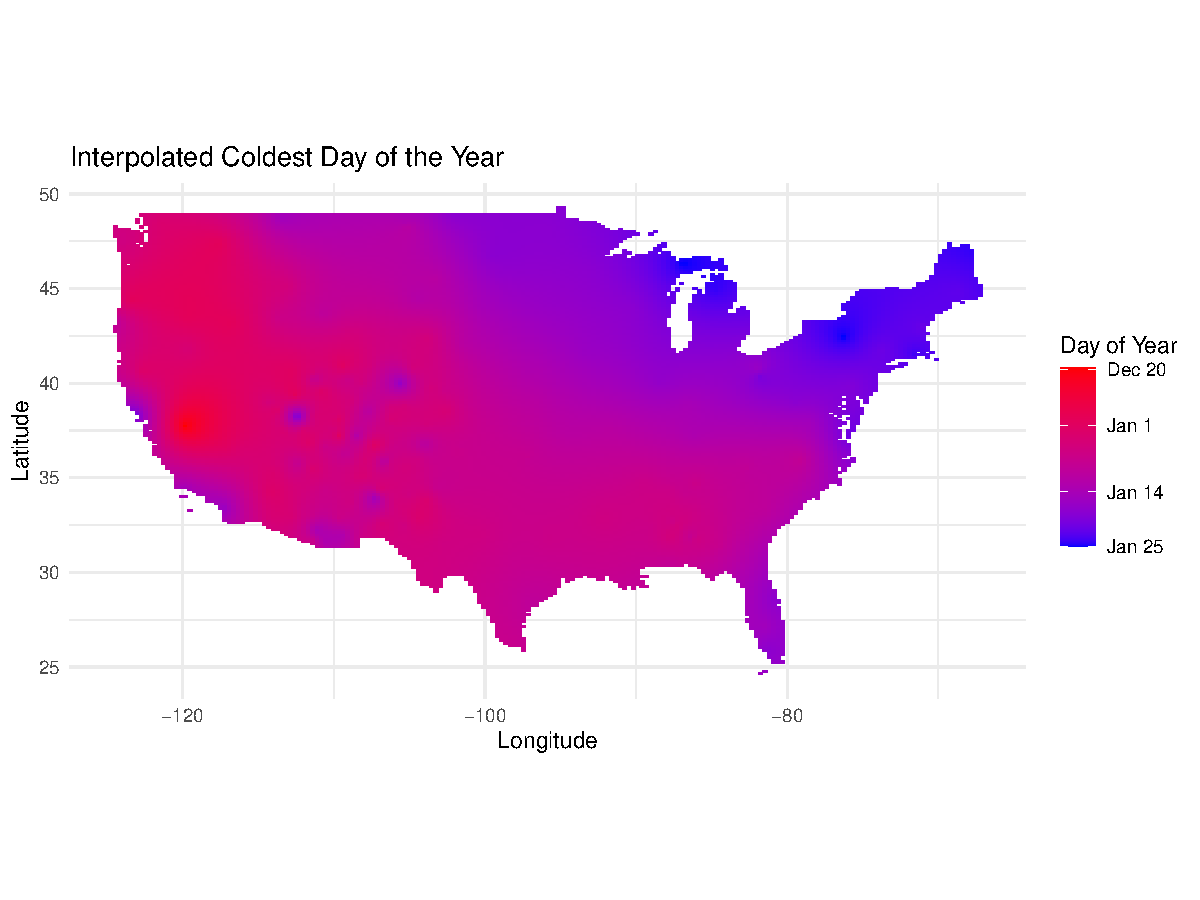
\includegraphics{seesaw_files/figure-latex/unnamed-chunk-8-2.pdf}

\begin{enumerate}
\def\labelenumi{\arabic{enumi}.}
\setcounter{enumi}{3}
\tightlist
\item
  Make a single plot of the estimated yearly cycles for 10 different
  stations, highlighting a diversity of climates around the contiguous
  USA. Your plot should clearly indicate which cycle is from which
  station.
\end{enumerate}

\begin{Shaded}
\begin{Highlighting}[]

\CommentTok{\# Select 10 stations from around the contiguous USA}
\CommentTok{\# ( Maine, Washington, Arizona, Wyoming, Oklahoma, Texas, Kentucky, Florida, }
\CommentTok{\#   Michigan, Pennsylvania )}
\NormalTok{stations }\OtherTok{\textless{}{-}} \FunctionTok{c}\NormalTok{(}\StringTok{"94645"}\NormalTok{, }\StringTok{"04223"}\NormalTok{, }\StringTok{"53169"}\NormalTok{, }\StringTok{"04131"}\NormalTok{, }\StringTok{"53182"}\NormalTok{, }\StringTok{"12987"}\NormalTok{, }\StringTok{"63849"}\NormalTok{, }
              \StringTok{"92826"}\NormalTok{, }\StringTok{"54810"}\NormalTok{, }\StringTok{"03761"}\NormalTok{)}
\NormalTok{states }\OtherTok{\textless{}{-}} \FunctionTok{c}\NormalTok{(}\StringTok{"Maine"}\NormalTok{, }\StringTok{"Washington"}\NormalTok{, }\StringTok{"Arizona"}\NormalTok{, }\StringTok{"Wyoming"}\NormalTok{, }\StringTok{"Oklahoma"}\NormalTok{, }\StringTok{"Texas"}\NormalTok{, }
           \StringTok{"Kentucky"}\NormalTok{, }\StringTok{"Florida"}\NormalTok{, }\StringTok{"Michigan"}\NormalTok{, }\StringTok{"Pennsylvania"}\NormalTok{)}
\CommentTok{\# Select 10 colors}
\NormalTok{cols }\OtherTok{\textless{}{-}} \FunctionTok{c}\NormalTok{(}\StringTok{"chartreuse1"}\NormalTok{, }\StringTok{"darkcyan"}\NormalTok{, }\StringTok{"dodgerblue4"}\NormalTok{, }\StringTok{"goldenrod1"}\NormalTok{, }\StringTok{"darkorange1"}\NormalTok{,}
          \StringTok{"deeppink3"}\NormalTok{, }\StringTok{"green4"}\NormalTok{, }\StringTok{"mediumpurple"}\NormalTok{, }\StringTok{"midnightblue"}\NormalTok{, }\StringTok{"firebrick3"}\NormalTok{)}
\CommentTok{\# Initialize plot}
\NormalTok{plt }\OtherTok{\textless{}{-}} \FunctionTok{ggplot}\NormalTok{() }\SpecialCharTok{+} 
  \FunctionTok{labs}\NormalTok{(}\AttributeTok{title =} \StringTok{"Estimated Yearly Cycles"}\NormalTok{, }
       \AttributeTok{x =} \StringTok{"DOY"}\NormalTok{, }\AttributeTok{y =} \StringTok{"Expected\_T\_DAILY\_AVG"}\NormalTok{)}
\CommentTok{\# Calculate and plot estimated yearly cycle for each station}
\ControlFlowTok{for}\NormalTok{ (i }\ControlFlowTok{in} \DecValTok{1}\SpecialCharTok{:}\DecValTok{10}\NormalTok{)\{}
\NormalTok{  cycle }\OtherTok{\textless{}{-}} \FunctionTok{yearly\_cycle\_station}\NormalTok{(stations[i])}
\NormalTok{  cycle}\SpecialCharTok{$}\NormalTok{state }\OtherTok{\textless{}{-}}\NormalTok{ states[i]}
\NormalTok{  plt }\OtherTok{\textless{}{-}}\NormalTok{ plt }\SpecialCharTok{+} \FunctionTok{geom\_line}\NormalTok{(}\AttributeTok{data =}\NormalTok{ cycle, }
                           \FunctionTok{aes}\NormalTok{(}\AttributeTok{x =}\NormalTok{ DOY, }\AttributeTok{y =}\NormalTok{ Expected\_T\_DAILY\_AVG,}
                               \AttributeTok{color =}\NormalTok{ state))}
\NormalTok{\}}
\CommentTok{\# Add legend}
\NormalTok{plt }\OtherTok{\textless{}{-}}\NormalTok{ plt }\SpecialCharTok{+} \FunctionTok{scale\_color\_manual}\NormalTok{(}\AttributeTok{name =} \StringTok{"State with Station"}\NormalTok{, }\AttributeTok{breaks =}\NormalTok{ states, }
                                \AttributeTok{values =} \FunctionTok{setNames}\NormalTok{(cols, states))}
\NormalTok{plt}
\end{Highlighting}
\end{Shaded}

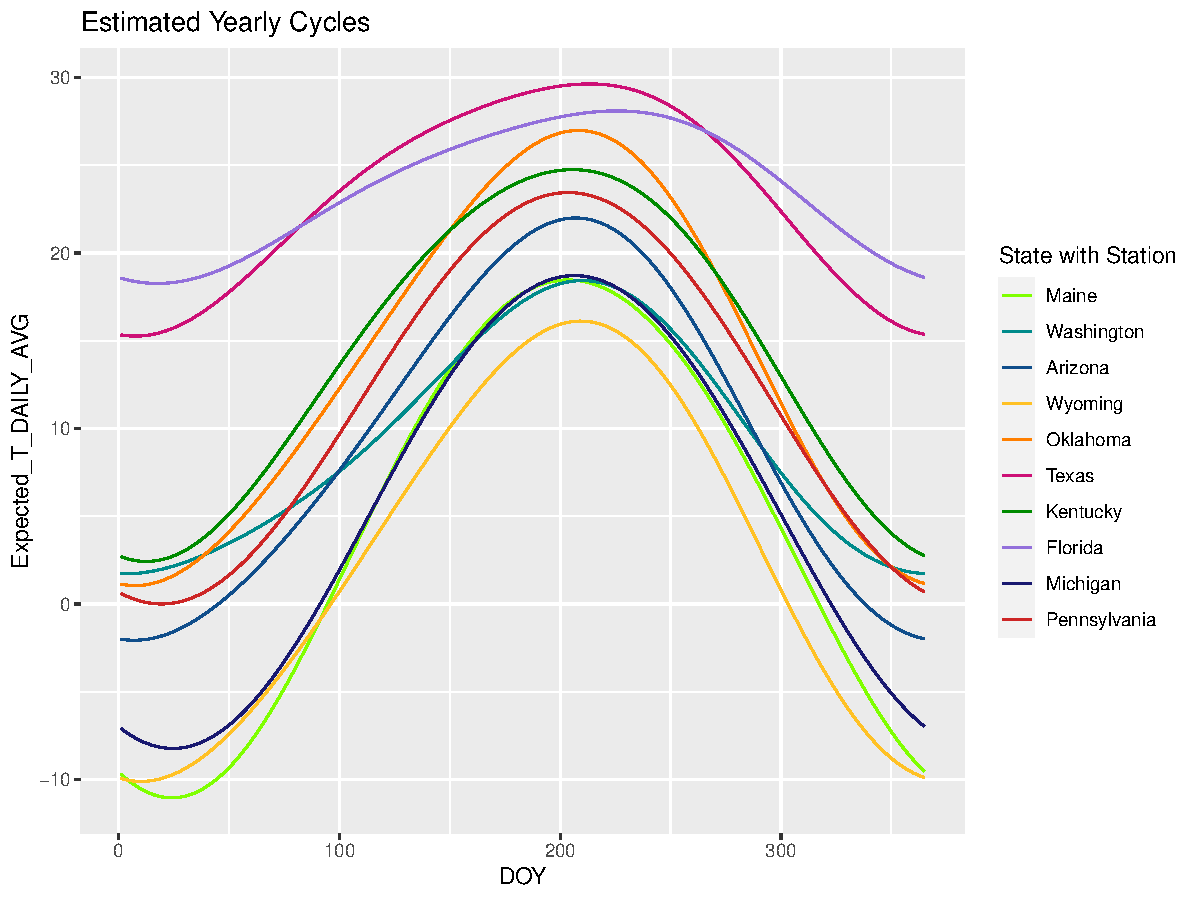
\includegraphics{seesaw_files/figure-latex/unnamed-chunk-9-1.pdf}

\begin{enumerate}
\def\labelenumi{\arabic{enumi}.}
\setcounter{enumi}{4}
\tightlist
\item
  Estimate the trend over the years for each station, in units of
  degrees Fahrenheit per year, and plot the trend values on a map.
  Indicate visually on your map which of the trends are statistically
  significant.
\end{enumerate}

In your report, write the statistical model that you used in
mathematical notation. Be sure to define all your symbols and
assumptions.

Interpolate the estimated trends to a grid, and plot them on a map. For
the interpolations, you may consider using only the trend estimates
whose standard errors are sufficiently small.

\begin{Shaded}
\begin{Highlighting}[]
\CommentTok{\# Find the temperature trends for each station (since 2000)}
\NormalTok{temp\_trends }\OtherTok{\textless{}{-}}  \FunctionTok{sapply}\NormalTok{(station\_info}\SpecialCharTok{$}\NormalTok{station\_id, seesaw}\SpecialCharTok{::}\NormalTok{trend\_of\_temps) }
\NormalTok{temp\_trends }\OtherTok{\textless{}{-}} \FunctionTok{t}\NormalTok{(temp\_trends)}

\CommentTok{\# Create a new data frame with station ids, temperature trend, lat and long}
\NormalTok{station\_trends }\OtherTok{\textless{}{-}} \FunctionTok{data.frame}\NormalTok{(}\AttributeTok{station\_id =} \FunctionTok{rownames}\NormalTok{(temp\_trends), }
                             \AttributeTok{trend =}\NormalTok{ temp\_trends[,}\DecValTok{1}\NormalTok{], }\AttributeTok{SE =}\NormalTok{ temp\_trends[,}\DecValTok{2}\NormalTok{])}
\CommentTok{\# Merge df with station\_info to get lat and lon}
\NormalTok{station\_trends }\OtherTok{\textless{}{-}} \FunctionTok{merge}\NormalTok{(station\_trends, station\_info, }\AttributeTok{by.x =} \StringTok{"station\_id"}\NormalTok{, }
                        \AttributeTok{by.y =} \StringTok{"station\_id"}\NormalTok{)}

\CommentTok{\# Determine which trends are statistically significant}
\NormalTok{sd }\OtherTok{\textless{}{-}} \FunctionTok{var}\NormalTok{(station\_trends}\SpecialCharTok{$}\NormalTok{trend, }\AttributeTok{na.rm =} \ConstantTok{TRUE}\NormalTok{)}
\NormalTok{n }\OtherTok{\textless{}{-}} \FunctionTok{length}\NormalTok{(station\_trends}\SpecialCharTok{$}\NormalTok{trend)}
\NormalTok{test\_statistics }\OtherTok{\textless{}{-}}\NormalTok{ (station\_trends}\SpecialCharTok{$}\NormalTok{trend }\SpecialCharTok{{-}} \DecValTok{0}\NormalTok{) }\SpecialCharTok{/}\NormalTok{ ( sd}\SpecialCharTok{/}\FunctionTok{sqrt}\NormalTok{(n) )}
\NormalTok{p\_vals }\OtherTok{\textless{}{-}} \FunctionTok{pt}\NormalTok{( test\_statistics, }\AttributeTok{df =}\NormalTok{ n }\SpecialCharTok{{-}} \DecValTok{1}\NormalTok{, }\AttributeTok{lower.tail =} \ConstantTok{FALSE}\NormalTok{ )}

\NormalTok{determine\_significance }\OtherTok{\textless{}{-}} \ControlFlowTok{function}\NormalTok{(pval)\{}
  
  \CommentTok{\# Assume all pvals are greater than 0.05}
\NormalTok{  signif }\OtherTok{\textless{}{-}} \StringTok{" "}
  \ControlFlowTok{if}\NormalTok{ (}\FunctionTok{is.na}\NormalTok{(pval) }\SpecialCharTok{||}\NormalTok{ pval }\SpecialCharTok{\textgreater{}} \FloatTok{0.05}\NormalTok{)\{}
    \FunctionTok{return}\NormalTok{(signif)}
\NormalTok{  \}}
  \CommentTok{\# Greater than 0.01, less than 0.05}
  \ControlFlowTok{if}\NormalTok{ (pval }\SpecialCharTok{\textless{}=} \FloatTok{0.05} \SpecialCharTok{\&}\NormalTok{ pval }\SpecialCharTok{\textgreater{}} \FloatTok{0.01}\NormalTok{) \{}
\NormalTok{    signif }\OtherTok{\textless{}{-}} \StringTok{"*"}
\NormalTok{  \} }\ControlFlowTok{else} \ControlFlowTok{if}\NormalTok{ (pval }\SpecialCharTok{\textless{}=} \FloatTok{0.01} \SpecialCharTok{\&}\NormalTok{ pval }\SpecialCharTok{\textgreater{}} \FloatTok{0.001}\NormalTok{) \{}
  \CommentTok{\# Greater than 0.001, less than 0.01}
\NormalTok{    signif }\OtherTok{\textless{}{-}} \StringTok{"**"}
\NormalTok{  \} }\ControlFlowTok{else} \ControlFlowTok{if}\NormalTok{ (pval }\SpecialCharTok{\textless{}=} \FloatTok{0.001}\NormalTok{) \{}
  \CommentTok{\# Less than 0.001}
\NormalTok{    signif }\OtherTok{\textless{}{-}} \StringTok{"***"}
\NormalTok{  \}}
  \FunctionTok{return}\NormalTok{(signif)}
\NormalTok{\}}

\NormalTok{station\_trends}\SpecialCharTok{$}\NormalTok{signif }\OtherTok{\textless{}{-}} \FunctionTok{sapply}\NormalTok{(p\_vals, determine\_significance)}


\CommentTok{\# Plot the USA shapefile}
\NormalTok{usa\_boundary }\OtherTok{\textless{}{-}} \FunctionTok{st\_crop}\NormalTok{(}\FunctionTok{st\_make\_valid}\NormalTok{(shp\_file), }\AttributeTok{xmin =} \SpecialCharTok{{-}}\DecValTok{125}\NormalTok{, }\AttributeTok{xmax =} \SpecialCharTok{{-}}\FloatTok{66.93457}\NormalTok{, }
                    \AttributeTok{ymin =} \FloatTok{22.396308}\NormalTok{, }\AttributeTok{ymax =} \FloatTok{49.384358}\NormalTok{)}

\NormalTok{station\_trends\_sf }\OtherTok{\textless{}{-}} \FunctionTok{st\_as\_sf}\NormalTok{(station\_trends, }
                              \AttributeTok{coords =} \FunctionTok{c}\NormalTok{(}\StringTok{"longitude"}\NormalTok{, }\StringTok{"latitude"}\NormalTok{), }
                              \AttributeTok{crs =} \FunctionTok{st\_crs}\NormalTok{(usa\_boundary))}
\NormalTok{coordinates }\OtherTok{\textless{}{-}} \FunctionTok{st\_coordinates}\NormalTok{(station\_trends\_sf)}
\NormalTok{station\_trends\_sf}\SpecialCharTok{$}\NormalTok{x }\OtherTok{\textless{}{-}}\NormalTok{ coordinates[,}\DecValTok{1}\NormalTok{]}
\NormalTok{station\_trends\_sf}\SpecialCharTok{$}\NormalTok{y }\OtherTok{\textless{}{-}}\NormalTok{ coordinates[,}\DecValTok{2}\NormalTok{]}

\CommentTok{\# Plot overall trends}
\NormalTok{signifs }\OtherTok{=} \FunctionTok{c}\NormalTok{(}\StringTok{" "}\NormalTok{, }\StringTok{"*"}\NormalTok{, }\StringTok{"**"}\NormalTok{, }\StringTok{"***"}\NormalTok{)}
\NormalTok{signif.codes }\OtherTok{\textless{}{-}} \FunctionTok{c}\NormalTok{(}\StringTok{"p \textgreater{} 0.05"}\NormalTok{, }\StringTok{"0.01 \textless{} p \textless{}= 0.05"}\NormalTok{, }\StringTok{"0.001 \textless{} p \textless{} 0.01"}\NormalTok{, }
                  \StringTok{"p \textless{} 0.001"}\NormalTok{)}
\FunctionTok{ggplot}\NormalTok{() }\SpecialCharTok{+}
  \FunctionTok{geom\_sf}\NormalTok{(}\AttributeTok{data =}\NormalTok{ usa\_boundary) }\SpecialCharTok{+}
  \FunctionTok{coord\_sf}\NormalTok{(}\AttributeTok{lims\_method =} \StringTok{"geometry\_bbox"}\NormalTok{) }\SpecialCharTok{+}
  \FunctionTok{geom\_point}\NormalTok{(}\AttributeTok{data =}\NormalTok{ station\_trends\_sf, }
             \FunctionTok{aes}\NormalTok{(}\AttributeTok{color =}\NormalTok{ trend, }\AttributeTok{x =}\NormalTok{ x, }\AttributeTok{y =}\NormalTok{ y, }\AttributeTok{shape =}\NormalTok{ signif), }
             \AttributeTok{size =} \DecValTok{1}\NormalTok{) }\SpecialCharTok{+} \FunctionTok{theme\_minimal}\NormalTok{() }\SpecialCharTok{+}
  \FunctionTok{labs}\NormalTok{(}\AttributeTok{title =} \StringTok{"Temperature Trends Since 2000"}\NormalTok{, }
       \AttributeTok{x =} \StringTok{"Longitude"}\NormalTok{, }\AttributeTok{y =} \StringTok{"Latitude"}\NormalTok{) }\SpecialCharTok{+}
  \FunctionTok{scale\_color\_gradient}\NormalTok{(}\AttributeTok{name =} \StringTok{"Trend (°C/Year)"}\NormalTok{, }\AttributeTok{low =} \StringTok{"blue"}\NormalTok{, }\AttributeTok{high =} \StringTok{"red"}\NormalTok{) }\SpecialCharTok{+}
  \FunctionTok{scale\_shape\_discrete}\NormalTok{(}\AttributeTok{name =} \StringTok{"Significance"}\NormalTok{, }\AttributeTok{breaks =}\NormalTok{ signifs, }
                                \AttributeTok{labels =}\NormalTok{ signif.codes) }\SpecialCharTok{+}
  \FunctionTok{theme}\NormalTok{(}\AttributeTok{plot.title =} \FunctionTok{element\_text}\NormalTok{(}\AttributeTok{hjust =} \FloatTok{0.5}\NormalTok{))}
\end{Highlighting}
\end{Shaded}

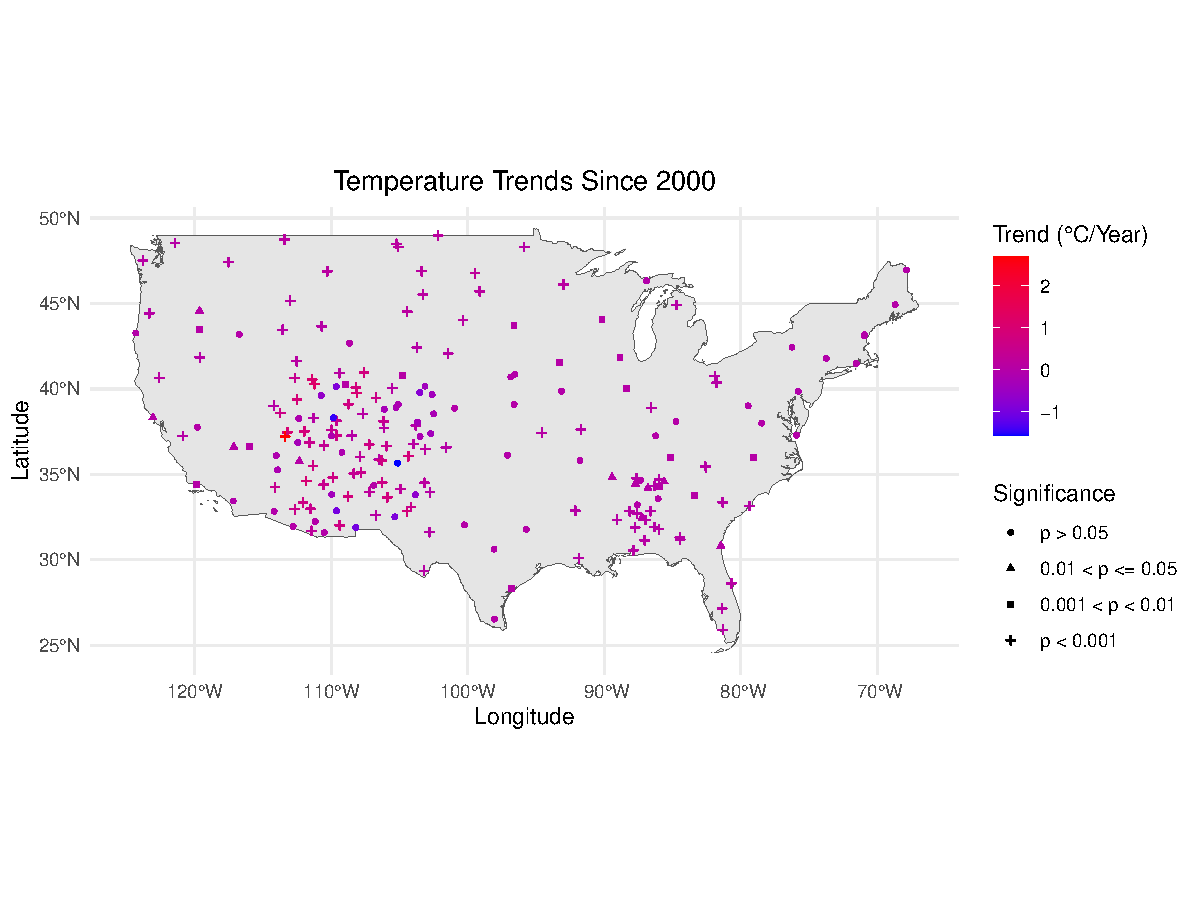
\includegraphics{seesaw_files/figure-latex/unnamed-chunk-10-1.pdf}

Statistical Model:

The estimated trend over the years for each station was calculated by
fitting a linear model for each month of the year and taking the average
of the slope coefficients from each linear model. This is given by:

\(estimated\ trend = \frac { \sum_{i = 1}^{12} \beta_{1i} }{12}\)

where \(\beta_{1i}\) denotes the slope coefficient for ith month, and is
derived from the model:

\(Y_i = \beta_0 + \beta_1 *d + \epsilon_i\)

where \(Y_i\) is the daily average temperature, \(d\) is the day of the
year, and \(\epsilon_i\) is the error term.

The standard error was found by converting the standard error of each
month's slope coefficient into a variance, pooling the variances, and
calculating the new standard error. That is,

\(Pooled\ Variance = \frac {\sum_{i=1}^{12}SE_i\ *\  n_i}{N - 12}\)
\textless\textless\textless\textless\textless\textless\textless{} HEAD

=======
\textgreater\textgreater\textgreater\textgreater\textgreater\textgreater\textgreater{}
7b390d4cc8e0fcfc9eb54c3fce5fa3b2484b7a8d
\(SE = \sqrt\frac {Pooled\ Variance}{N}\)

where \(SE_i\) is the standard error for the ith month, \(n_i\) is the
number of available readings for the 1st of that month at that station,
and \(N\) is the total sample size (total number of available readings
for the 1st of all months between the start and end dates at that
station).

Assumptions: 1. The change in temperature over the years can be modeled
linearly. Further, we assume that the the change in monthly temperatures
overall the years follows a linear trend as well. 2. The overall trend
for each month contributes equal to the station's trend overall (that
is, each month's trend is equally indicative of the trend overall) 3.
The error term is normally distributed with mean 0 and constant
variance.

To determine statistical significance, we assume that the temperature
trends of stations are normally distributed with mean 0, indicating the
temperature has not changed over the years. We run a t-test with
significance level \(\alpha = 0.05\) to determine which trends are
significant.

\begin{Shaded}
\begin{Highlighting}[]

\NormalTok{res }\OtherTok{\textless{}{-}} \DecValTok{100}

\CommentTok{\# Subset station\_trends to only include significant trends}
\NormalTok{significant\_trends }\OtherTok{\textless{}{-}}\NormalTok{ station\_trends[station\_trends}\SpecialCharTok{$}\NormalTok{signif }\SpecialCharTok{!=} \StringTok{" "}\NormalTok{,]}

\CommentTok{\# Interpolate trends for contiguous US}
\NormalTok{y }\OtherTok{\textless{}{-}}\NormalTok{ significant\_trends}\SpecialCharTok{$}\NormalTok{trend}
\NormalTok{locs }\OtherTok{\textless{}{-}}\NormalTok{ significant\_trends[, }\FunctionTok{c}\NormalTok{(}\StringTok{"longitude"}\NormalTok{, }\StringTok{"latitude"}\NormalTok{)]}
\FunctionTok{names}\NormalTok{(locs) }\OtherTok{\textless{}{-}} \FunctionTok{c}\NormalTok{(}\StringTok{"x"}\NormalTok{, }\StringTok{"y"}\NormalTok{)}
\NormalTok{locs}\SpecialCharTok{$}\NormalTok{x }\OtherTok{\textless{}{-}} \FunctionTok{as.numeric}\NormalTok{(locs}\SpecialCharTok{$}\NormalTok{x)}
\NormalTok{locs}\SpecialCharTok{$}\NormalTok{y }\OtherTok{\textless{}{-}} \FunctionTok{as.numeric}\NormalTok{(locs}\SpecialCharTok{$}\NormalTok{y)}
\NormalTok{X }\OtherTok{\textless{}{-}} \FunctionTok{as.data.frame}\NormalTok{(}\FunctionTok{cbind}\NormalTok{(}\DecValTok{1}\NormalTok{, locs))}

\NormalTok{grid }\OtherTok{\textless{}{-}} \FunctionTok{usagrid}\NormalTok{(res)}
\CommentTok{\# Make predictions}
\NormalTok{trend\_preds }\OtherTok{\textless{}{-}} \FunctionTok{interpolate\_grid}\NormalTok{(X,y,}\AttributeTok{resolution =}\NormalTok{ res)}
\CommentTok{\#\textgreater{} Assuming columns 1 and 2 of locs are (longitude,latidue) in degrees}

\CommentTok{\# Plot interpolations}
\FunctionTok{graph\_interp}\NormalTok{(trend\_preds, grid) }\SpecialCharTok{+} 
  \FunctionTok{labs}\NormalTok{( }\AttributeTok{title =} \StringTok{"Interpolated Trend Over the Years"}\NormalTok{,}
    \AttributeTok{x =} \StringTok{"Longitude"}\NormalTok{, }\AttributeTok{y =} \StringTok{"Latitude"}\NormalTok{, }
    \AttributeTok{fill =} \StringTok{"Trend (°C/Year)"}\NormalTok{)}
\end{Highlighting}
\end{Shaded}

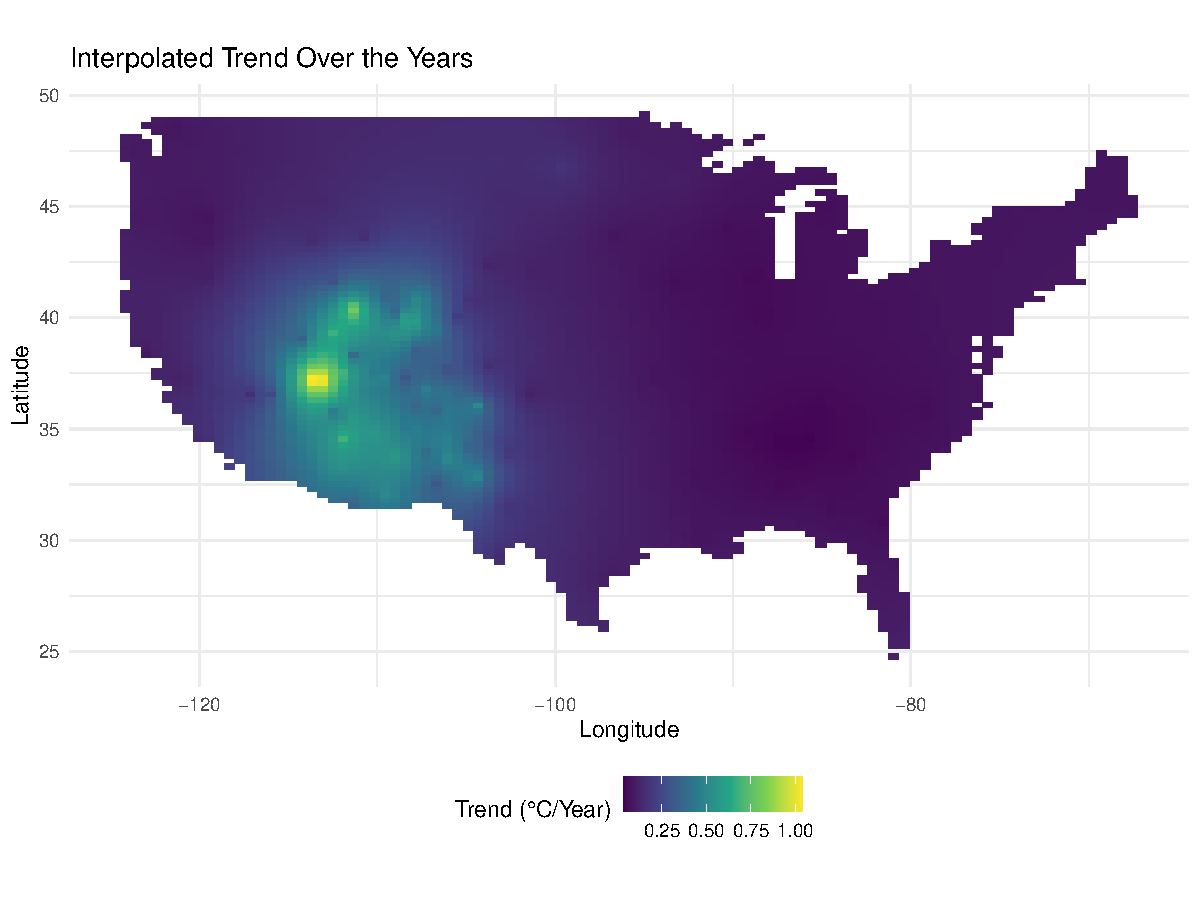
\includegraphics{seesaw_files/figure-latex/unnamed-chunk-11-1.pdf}

\begin{enumerate}
\def\labelenumi{\arabic{enumi}.}
\setcounter{enumi}{5}
\tightlist
\item
  Find a reputable source for the average temperature trend in the
  contiguous USA over the past 20 years, and compare your results to the
  source's.
\end{enumerate}

Reputable Source: US EPA
\url{https://www.epa.gov/climate-indicators/climate-change-indicators-us-and-global-temperature}

\begin{Shaded}
\begin{Highlighting}[]
\FunctionTok{median}\NormalTok{(significant\_trends}\SpecialCharTok{$}\NormalTok{trend)}\SpecialCharTok{*}\DecValTok{10}
\CommentTok{\#\textgreater{} [1] 0.7349643}
\end{Highlighting}
\end{Shaded}

The EPA reports that the average temperature in the contiguous US has
risen by 0.55°F per decade since 1981. This is equivalent to 0.306°C per
decade. Our model estimates the average temperature trend in the
contiguous US to be roughly 0.73°C per decade. However, this is largely
due to the fact that we are only considering the temperature trends
since 2000, where according to the EPA, temperature has been increasing
even faster. Additionally, it is the case that the vast majority of the
US is increasing at a rate lower than 0.73°C per decade, while stations
in the Southwest are increasing at a much greater rate.

\end{document}
